\documentclass{report}
% 导言区
\usepackage{amsmath}
\usepackage{xeCJK}
\usepackage{graphicx}
\graphicspath{{figures/}}
\usepackage[scale=0.8]{geometry}
\usepackage{float}
\usepackage{amsmath}
%\usepackage{hypertoc}
\usepackage{hyperref}
\usepackage{array}
\usepackage{setspace}
\usepackage{xcolor}
\usepackage{setspace}

% 自定义命令
\newcommand{\clearquestion}{
	\setcounter{question}{0}
}
\newcounter{question}[section]
\newcommand{\question}[1]{
	\stepcounter{question}
	\paragraph{\thequestion \hspace{0.5em} #1 }
}
% 自定义无缩进
%\renewcommand{\noindent}{\setlength\parindent{0em}}
% 设置行距
\renewcommand{\baselinestretch}{1.0}
% 加深编号
\setcounter{secnumdepth}{3}

\begin{document}
	\chapter{概论}
%\section{基础}
\vspace{-5em}
\noindent\question{信息系统的脆弱性主要体现在以下几个方面:}
\begin{enumerate}
	\item 物理因素,物理设备的自然、人为破坏。
	\item 网络因素,信息系统软件复杂度越来越高。
	\item 系统因素,信息系统软件复杂度越来越高
	\item 应用因素,不正确的操作和人为的蓄意破坏。
	\item 管理因素,管理制度、法律不健全。
\end{enumerate}
\question{信息安全的目标:}对网络中的硬件、软件和系统中的数据进行保护,不受偶然或者恶意的因素影响而遭到破坏、更改、泄漏,使系统能稳定可靠正常地运行,使信息服务不中断。

\question{信息安全关注的几点问题:}
\begin{enumerate}
	\item 密码理论与技术
	\item 安全协议理论与技术
	\item 安全体系结理论与技术
	\item 信息对抗理论与技术
	\item 网络安全与安全产品
\end{enumerate}

\question{互联网络的特点:}
\begin{enumerate}
	\item 无中心网,再生能力强
	\item 可实现移动通信、多媒体通信等多种服务
	\item 互联网一般分为外部网和内部网
	\item 互联网的用户主体是个人
\end{enumerate}
%\section{安全模型}
%\subsection{ P2DR 模型}
\question{P2DR 模型}
\begin{itemize}
	\item Policy 安全策略
	\item Protection 防护
	\item Detection  检测
	\item Response 响应
\end{itemize}
%\subsection{ PDRR 模型}
\question{PDRR模型}
\begin{itemize}
	\item Protection 防护
	\item Detection 检测
	\item Response 响应
	\item Recovery 恢复
\end{itemize}
%\section{安全体系结构}
\question{ISO开方系统互联安全体系的五类安全服务}
\begin{enumerate}
	\item 鉴别服务
	\item 访问控制服务
	\item 数据机密性服务
	\item 数据完整性服务
	\item 抵抗性
\end{enumerate}
	\chapter{密码学概论}

\question{RSA算法}\\
公钥与密钥的产生
\begin{enumerate}
	\item 随意选择两个大的质数p和q,p不等于q,计算N=pq。
	\item 根据欧拉函数,求得r = (p-1)(q-1)
	\item 选择一个小于 r 的整数 e,求得 e 关于模 r 的模反元素,命名为d。(模反元素存在,\textbf{当且仅当e与r互质})
	\begin{equation}\label{key}
	e\times d = 1\ mod\ r
	\end{equation}
	\item 将 p 和 q 的记录销毁。
\end{enumerate}
(N,e)为公钥,(N,d)为私钥。\textbf{采用公钥加密,私钥解密}\\
一个实例
\begin{gather}
 p = 3,q=11 , N = pq = 33\\
 r = (p-1)(q-1) = 2*10 = 20 \\
 ed = r * n + 1\\
 e = 3,d = 7\\
\end{gather}
所以公钥(33,3),私钥(33,7)。要传输的消息m = 24
\begin{gather}
 \text{加密}\quad m^e mod N = 24^3 \% 33 = 30\\
 \text{解密}\quad c^d mod N = 30 ^d \% 33 =24
\end{gather}

	\chapter{数字签名与身份认证}

\question{计算机安全的四大原则},机密性、完整性、可认证性、不可抵赖性。

\question{安全协议}
\begin{enumerate}
	\item 以密码学为基础
	\item 也是通信协议
\end{enumerate}
分类:
\begin{enumerate}
	\item 密钥生成协议
	\item 认证协议
	\item 电子商务协议
	\item 安全多方计算协议
\end{enumerate}

\question{数字签名},\textbf{基于非对称密码算法},是一串数据,该数据仅能由签名人生成,并且该数据能够表明签名人的身份。一般由两个部分组成
\begin{enumerate}
	\item 签名算法,由签名方秘密保存
	\item 验证算法,通常是公开的,便于他人验证签名的有效性
\end{enumerate}
通常分为两类:
\begin{enumerate}
	\item 直接数字签名
	\item 基于仲裁的数字签名
\end{enumerate}

\question{数字签名算法}
\begin{enumerate}
	\item DSA
	\begin{figure}[H]
		\centering
		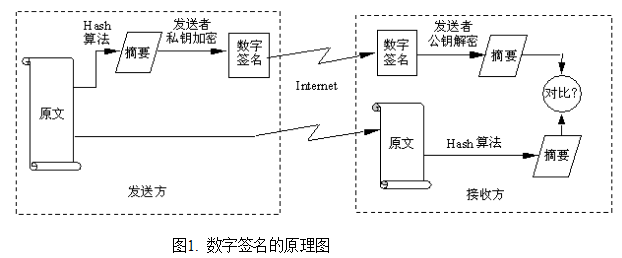
\includegraphics[width=0.7\linewidth]{dsa.png}
	\end{figure}
	\begin{enumerate}
		\item 使用SHA编码将发送文件加密产生128bit的数字摘要; 
		\item 发送方用自己的专用密钥对摘要再加密,形成数字签名; 
		\item 将原文和加密的摘要同时传给对方; 
		\item 接受方用发送方的公共密钥对摘要解密,同时对收到的文件用SHA编码加密产生同一摘要; 
		\item 将解密后的摘要和收到的文件在接受方重新加密产生的摘要相互对比,如果两者一致,则说明在传送过程中信息没有破坏和篡改。否则,则说明信息已经失去安全性和保密性。
	\end{enumerate}
\end{enumerate}
	\chapter{PKI技术}
\question{PKI 的概念及作用}
PKI是一个用\textbf{非对称密码算法}原理和技术来实现并\textbf{提供安全服务}的
具有通用性的安全基础设施。能够为所有网络应用提供采用加密
和数字签名等密码服务所需要的\textbf{密钥和证书管理}。

\question{为什么需要PKI?}
在网络、信息系统上,需要统一的、安全的认证技术

\question{提供的服务}
\begin{enumerate}
	\item 认证:PKI 通过证书进行认证,这个证书是一个可信的第三方证明的,通过它,通信双方可以安全地进行互相认证,而
	不用担心对方是假冒的。
	\item 数据保密:通过加密证书,通信双方可以协商一个密钥,而这个密钥可以作为通信加密的密钥。
	\item 完整性与不可否认:通过数字签名和可信的第三方仲裁来保证完整性和不可否认。
\end{enumerate}
\question{证书内容}
1、版本信息 2、序列号 3、签名算法 4、发行机构 5、有效期 6、拥有者 7、公开密钥 8、签名
\question{PKI的组成}
\begin{itemize}
	\item PKI 策略
	\item 软硬件系统 
	\item 注册机构(RA) 
	\item 认证中心(CA) \textbf{核心}
	\item 证书签发系统 
	\item PKI 应用 
	\item PKI 应用接口系统
\end{itemize}

\question{PKI 互通的实现途径}
\begin{enumerate}
	\item 根CA之间的交叉认证。桥接
	\item 全球性统一根CA。代理
\end{enumerate}
	\chapter{防火墙}
%\clearquestion
\question{什么是防火墙}
防火墙是一种协助确保信息安全的设施,\textbf{依照特定的规则},允许或是禁止传输的数据通过。

\question{防火墙放置位置}
位于信任内部网络和不可信任的外界网络之间,如网关,防火墙主机上的一些特定的应用程序。

\question{防火墙的特性}
\begin{enumerate}
	\item 内部网络和外部网络之间的所有网络数据都必须经过防火墙
	\item 只有符合安全策略的数据流才能通过防火墙
	\item 防火墙自身应具有非常强的抗攻击免疫力
\end{enumerate}

\question{防火墙的功能}
\begin{enumerate}
	\item 防火墙是网络安全的屏障
	\item 防火墙可以强化网络安全策略
	\item 防火墙可以对网络存取和访问进行监控审计
	\item 防火墙可以防范内部消息的外泄
\end{enumerate}

\question{防火墙网络层的性质指标}
\begin{enumerate}
	\item 吞吐量指标
	\item 时延指标
	\item 丢包率指标
	\item 背靠背缓冲指标
\end{enumerate}

\question{防火墙常见的功能指标}
\begin{enumerate}
	\item 服务平台支持
	\item LAN口支持
	\item 协议支持
	\item VPN支持
	\item \dots
\end{enumerate}

\question{防火墙核心技术}
\begin{enumerate}
	\item 包过滤技术,在\textbf{网络层}截获网络数据包,根据防火墙的规则表,来检测攻击行为,在网络层提供较低级别的安全防护和控制
	\item 应用网关技术,又被成为代理技术,位于应用层上,所以主要采用协议代理服务。应用代理防火墙壁分组过滤防火墙提供更高层次的安全性,但这丧失对应用程序的透明性。
	\item 状态检测技术,采用一种基于连接的状态监测机制,将属于同一连接的所有包作为一个整体的数据流看待,构成连接状态表,通过规则表与状态的共同配置,对表中的各个连接状态因素加以识别。\textbf{是一种动态的判定方法。(前两种为静态)}Steps:
	\begin{itemize}
		\item 检查是否属于一个已建立的连接
		\item 若已建立,则根据连接状态表的策略对数据包实施丢弃、拒绝或是转发。
		\item 若未建立连接,会检查数据包是否与他配置的规则集匹配。
	\end{itemize}
\end{enumerate}

\question{防火墙分类}
\begin{enumerate}
	\item 个人防火墙
	\item 分布式防火墙
	\item 分层式防火墙
\end{enumerate}

\question{防火墙的体系结构,部署位置}
\hspace{2em}\\
基本概念:
\begin{enumerate}
	\item 堡垒主机,一种被强化的可以防御攻击的计算机,作为进入内部网络的一个检查点。堡垒主机是网络中\textbf{最容易受到侵害}的主机。\textbf{包过滤路由器和应用代理服务器均可视为堡垒主机。}
	\item 非军事区,也成为“隔离区”,他是为了解决安装防火墙后,外部网络不能访问内部网络服务器的问题,而设立的一个非安全系统与安全系统之间的缓冲区。
\end{enumerate}
体系结构分类:
\begin{enumerate}
	\item 筛选路由器体系结构。
	\item 单宿主堡垒主机,由包过滤路由器和堡垒主机构成。外部路由器配置把所有进来的数据发送到堡垒主机上,所有出去的数据包也经过堡垒主机(代理)。实现了网络层安全(包过滤)和应用层安全(代理服务)。缺点:可通过重新配置路由器,使数据绕过堡垒主机。
	\item 双宿主堡垒主机,与单宿主堡垒主机的区别在于,双宿主堡垒主机有两块网卡,一块连接内部网络,一块连接包过滤路由器,但是主机两个端口之间直接转发信息的功能被关闭。在应用层提供代理服务
	\item 屏蔽子网体系结构:由两个包过滤路由器和一个堡垒主机构成,支持网络层和应用层的安全功能。在定义非军事区(DMZ),即屏蔽子网后。存在内部防火墙和外部防火墙。攻击者要通过外部防火墙,堡垒主机和内部防火墙三道防线,才能到达内部网络。
	\begin{figure}[H]
		\centering
		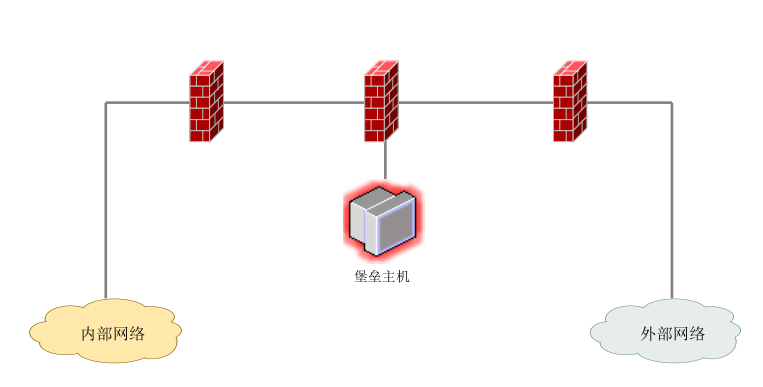
\includegraphics[width=0.7\linewidth]{figures/screenshot001}
		\caption{}
		\label{fig:screenshot001}
	\end{figure}
\end{enumerate}

\question{常见产品}
\begin{enumerate}
	\item Firewall
	\item PIX
	\item AXENT Raptor
	\item NetScreen
	\item 天融信网络卫士
	\item 东软NetEye  4032防火墙
\end{enumerate}






\end{document}